\section{Related Work}

\subsection{Toolpath strategies}

\todo{Find reference on patchwise Zig-Zag toolpathing strategy.}

Combining concentric toolpaths into continuous extrusion spirals. \cite{Held2009}

Defining a continuous extrusion Zig-Zag toolpath. \cite{Jin2017}

\subsection{Space filling toolpaths}
\todo{find other literature which tries to minimize underfilling and overfilling which is not based on a skeletonization.}


\subsection{Medial axis based toolpaths}
Adjusted Medial Axis Transform (MAT) structure for only printing the outer wall, rest area to be filled using normal infill. \cite{Moesen2011}
\Cref{moessen}
Problem: small grey areas which are too small for the second wall lines.

Figuring out underfilling and overfilling arteas in concentric fill and using single squigly lines to prevent overfilling. \cite{Jin2017}
\Cref{jin}

Using variable width lines to fit a precise amount of lines using the MAT.
\cite{Ding2016a} apply the method from \cite{kao1998optimal}.
\Cref{ding}

\begin{figure}
\begin{subfigure}{0.45\columnwidth}
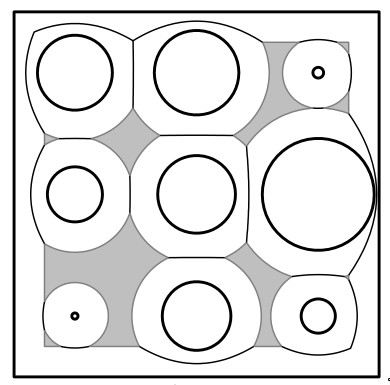
\includegraphics[width=\columnwidth]{sources/related_work/moessen.jpg}
\caption{\citeauthor{Moesen2011}}
\label{moessen}
\end{subfigure}
\begin{subfigure}{0.45\columnwidth}
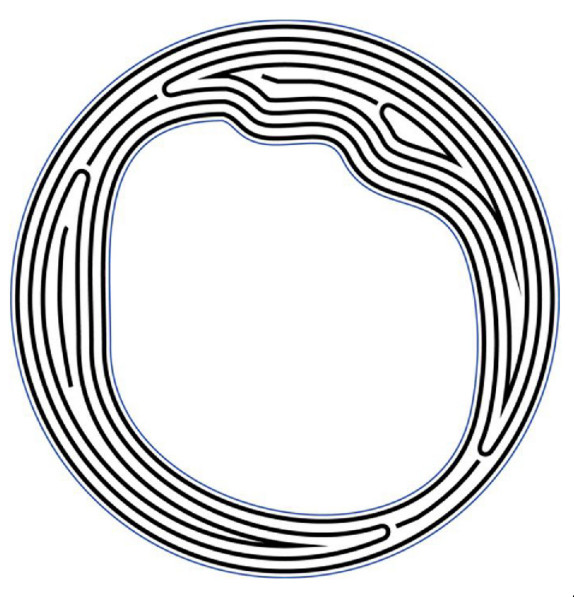
\includegraphics[width=\columnwidth]{sources/related_work/jin.jpg}
\caption{\citeauthor{Jin2017}}
\label{jin}
\end{subfigure}
\end{figure}

\begin{figure}
\centering
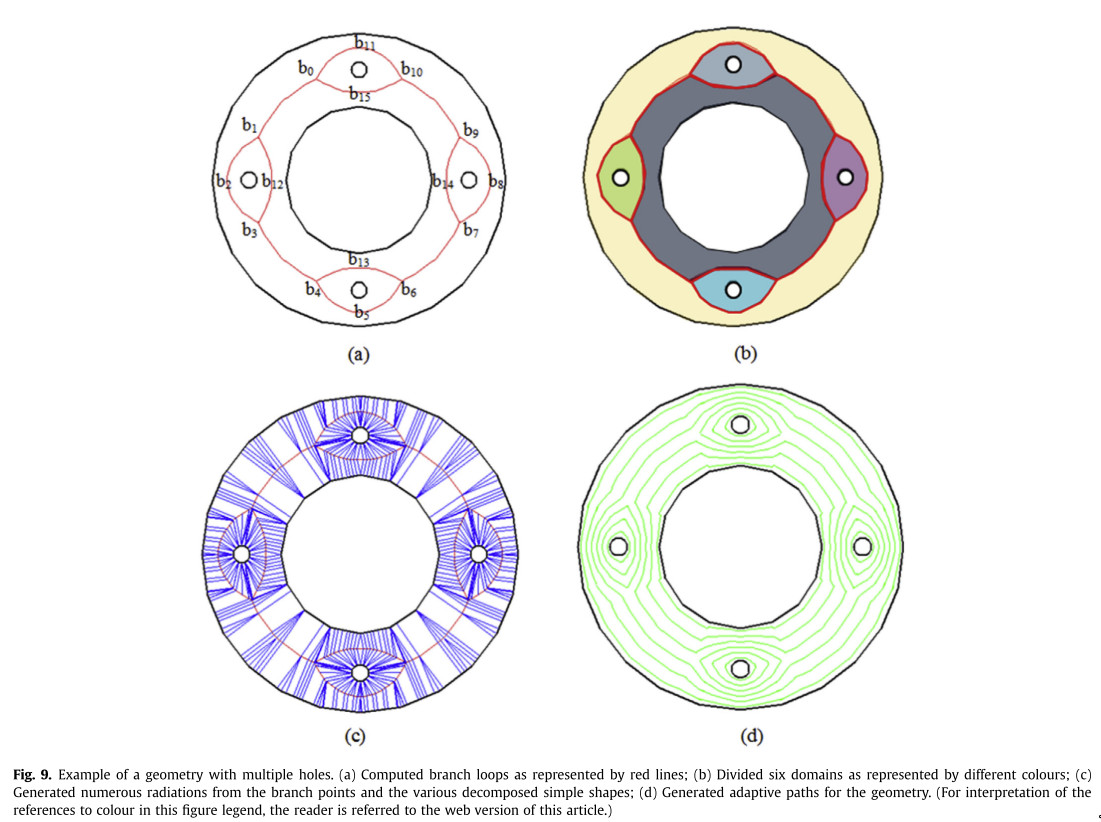
\includegraphics[width=\columnwidth]{sources/related_work/ding.jpg}
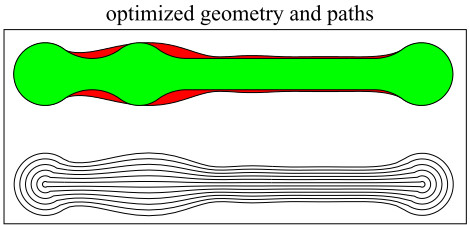
\includegraphics[width=.7\columnwidth]{sources/related_work/kao.jpg}
\caption{Path planning strategies proposed by Kao (bottom) and employed in FDM by Ding et al (top).}
\label{ding}
\end{figure}

\subsection{Variable extrusion width}

Changing extrusion rate and temperature to match a given velocity. \cite{Ertay2018}

Changing velocity in order to change extrusion rate.
Shortly discussed in \cite{Kuipers2018}.
\todo{find another reference}